% !TEX program = xelatex
% 공통수학2 · Ⅰ. 도형의 방정식 · 2. 원의 방정식 · 02 원과 직선의 위치 관계 · 1/2차시
% 학생용 활동지 (답안 없음)
\documentclass[11pt,a4paper]{article}
\usepackage{kotex}
\usepackage{iftex}
\ifPDFTeX\else
  \setmainhangulfont{Noto Serif CJK KR}
  \setsanshangulfont{Noto Sans CJK KR}
\fi
\usepackage[margin=2.1cm]{geometry}
\usepackage{parskip}
\usepackage{enumitem}
\usepackage{array}
\usepackage{tabularx}
\usepackage{xcolor}
\usepackage{amssymb}
\usepackage{tikz}
\usepackage[most]{tcolorbox}
\usepackage{fancyhdr}
\usepackage{titlesec}

\definecolor{goldc}{HTML}{B07C22}
\definecolor{goldstrong}{HTML}{8A5F16}
\definecolor{indigoc}{HTML}{2B3B57}
\definecolor{indigosoft}{HTML}{6E82A6}
\definecolor{linec}{HTML}{D6DACB}
\definecolor{surface2}{HTML}{E4E8DC}
\definecolor{writeline}{HTML}{C7CCBA}
\definecolor{inksoft}{HTML}{52604F}

\titleformat{\section}{\normalfont\sffamily\bfseries\large\color{indigoc}}{\thesection}{0.6em}{}
\titlespacing{\section}{0pt}{14pt}{6pt}
\newtcolorbox{goalbox}{enhanced, breakable, colback=white, colframe=goldc, boxrule=0.5pt, leftrule=3pt, arc=2pt, left=10pt, right=10pt, top=8pt, bottom=8pt}
\newtcolorbox{sheetbox}{enhanced, breakable, colback=white, colframe=linec, boxrule=0.6pt, arc=3pt, left=11pt, right=11pt, top=9pt, bottom=9pt}
\newcommand{\writespace}[1]{%
  \par\nobreak\vspace{3pt}
  \foreach \n in {1,...,#1} {%
    \noindent\textcolor{writeline}{\rule{\linewidth}{0.4pt}}\par\vspace{0.62cm}%
  }
}
\newcommand{\fillblank}[1]{\makebox[#1]{\hrulefill}}
\pagestyle{fancy}\fancyhf{}\renewcommand{\headrulewidth}{0pt}
\fancyfoot[L]{\footnotesize\color{inksoft} 공통수학2 · 2026학년도 2학기 · 지평선고등학교}
\fancyfoot[R]{\footnotesize\color{inksoft} 다음 시간 --- 02 원과 직선의 위치 관계(2) 접선}

\begin{document}

\noindent
\begin{minipage}[b]{0.62\linewidth}
  {\sffamily\footnotesize\color{indigosoft} 공통수학2 · Ⅰ. 도형의 방정식 · 2. 원의 방정식}\\[2pt]
  {\sffamily\bfseries\Large 02 원과 직선의 위치 관계 \textperiodcentered\ 11차시}
\end{minipage}\hfill
\begin{minipage}[b]{0.36\linewidth}
  \raggedleft\small\color{inksoft}
  반\ \fillblank{1.6cm} \quad 번호\ \fillblank{1.6cm}\\[4pt]
  이름\ \fillblank{3.6cm}
\end{minipage}

\vspace{4pt}
\noindent{\color{goldc}\rule{\linewidth}{2.2pt}}
\vspace{10pt}

\begin{goalbox}
\textbf{오늘의 목표}\\
원과 직선의 방정식을 연립하여 얻은 판별식으로, 또는 중심과 직선 사이의 거리로 위치 관계를 판단할 수 있다.
\vspace{4pt}
\small\color{inksoft}
$\square$ 자신 있음 \quad $\square$ 조금 헷갈림 \quad $\square$ 처음 봄 \hfill (수업 전 나의 상태에 표시)
\end{goalbox}

\section{생각 열기 --- 원과 직선, 몇 번 만날까?}

\begin{sheetbox}
반지름의 길이가 $r$인 원과 직선이 있다. 원의 중심 O와 직선 사이의 거리를 $d$라 하자.

\begin{center}
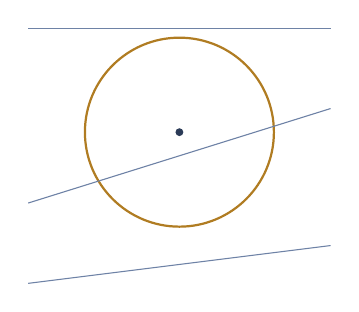
\begin{tikzpicture}[scale=0.6]
  \draw[thick, goldc] (0,0) circle (2);
  \filldraw[indigoc] (0,0) circle (2pt);
  \draw[thin, indigosoft] (-3.2,-1.5) -- (3.2,0.5);
  \draw[thin, indigosoft] (-3.2,2.2) -- (3.2,2.2);
  \draw[thin, indigosoft] (-3.2,-3.2) -- (3.2,-2.4);
\end{tikzpicture}
\end{center}

\begin{enumerate}[leftmargin=1.4em, itemsep=3pt]
  \item $d \fillblank{1.2cm} r$일 때, 서로 다른 두 점에서 만난다.
  \item $d \fillblank{1.2cm} r$일 때, 한 점에서 만난다(접한다).
  \item $d \fillblank{1.2cm} r$일 때, 만나지 않는다.
\end{enumerate}
\end{sheetbox}

\section{개념 정리 --- 판별식으로 판단하기}

\begin{sheetbox}
원 $x^2+y^2=r^2$과 직선 $y=mx+n$을 연립하면
\[
(m^2+1)x^2+2mnx+(n^2-r^2)=0
\]
이 이차방정식의 판별식을 $D$라 하면,

\begin{enumerate}[leftmargin=1.6em, itemsep=3pt]
  \item $D \fillblank{1.2cm} 0$이면 서로 다른 두 점에서 만난다.
  \item $D \fillblank{1.2cm} 0$이면 한 점에서 만난다(접한다).
  \item $D \fillblank{1.2cm} 0$이면 만나지 않는다.
\end{enumerate}

\vspace{4pt}
\textbf{보기} --- 원 $x^2+y^2=16$과 직선 $y=x-2$의 위치 관계를 판별식으로 확인해 보자.
\writespace{3}
\end{sheetbox}

\section{연습 문제}

\begin{sheetbox}
\textbf{1.} 다음 원과 직선의 위치 관계를 두 가지 방법(판별식, 거리 비교) 중 하나로 말하시오.\\
\hspace*{1.6em}⑴ $x^2+y^2=1$, $y=-2x+3$ \qquad ⑵ $x^2+y^2=8$, $x+y=4$
\writespace{5}

\vspace{6pt}
\textbf{2.} 원 $x^2+y^2=4$와 직선 $y=2x+k$가 만나지 않도록 하는 실수 $k$의 값의 범위를 구하시오.
\writespace{3}
\end{sheetbox}

\section{사고의 가시화 --- See · Think · Wonder}

\noindent{\footnotesize\color{inksoft} 오늘 배운 `원과 직선의 위치 관계'를 떠올리며 아래 세 칸을 채워 보자.}\\[6pt]
\begin{tabularx}{\linewidth}{@{}XXX@{}}
\textbf{\footnotesize\color{indigoc} See --- 무엇을 보았나?} &
\textbf{\footnotesize\color{indigoc} Think --- 무엇을 생각했나?} &
\textbf{\footnotesize\color{indigoc} Wonder --- 무엇이 궁금한가?} \\[4pt]
\end{tabularx}
\noindent
\begin{minipage}[t]{0.32\linewidth}\writespace{3}\end{minipage}\hfill
\begin{minipage}[t]{0.32\linewidth}\writespace{3}\end{minipage}\hfill
\begin{minipage}[t]{0.32\linewidth}\writespace{3}\end{minipage}

\section{마무리 성찰}

\begin{sheetbox}
\begin{minipage}[t]{0.48\linewidth}
{\footnotesize\color{inksoft} 오늘 배운 것을 한 문장으로}
\writespace{2}
\end{minipage}\hfill
\begin{minipage}[t]{0.48\linewidth}
{\footnotesize\color{inksoft} 감사 일기 / 유념 한 줄}
\writespace{2}
\end{minipage}
\end{sheetbox}

\end{document}
